\chapter{Deep Declarative Network}
\label{cha:ddn}
In this chapter, we will cover the structure and nodes in the deep declarative network: from its learning process to the back-propagation.
\par Before delving into the details of the back-propagation in different constraints cases, we give an overview of the deep declarative network in Section~\ref{sec:overview-ddn}. In particular, the basic structure of the network and the details of declarative nodes are described according to \cite{SG:19}. The learning progress of the network is also given. We hope this will give readers a better sense of what is the deep declarative network and how it works. 
\par In Section~\ref{sec:bp}, we present the details of the back-propagation in different constrained problems. The gradient computation results are based on the implicit differentiation and different in constrained problems. We discuss this part based on the regular solution and compare it with the general solution in the previous chapter. 
\par Next we present the examples of constrained optimization problems with both linear and non-linear, equality and inequality constraints in Section~\ref{sec:example}. We also provide more implementation details of the deep declarative nodes. 
\par Finally, we summarize the deep declarative network and its solution in different constrained problems under the regular point. 


\section{An Overview of Deep Declarative Network}
\label{sec:overview-ddn}
\subsection{Declarative Node}
In deep declarative network, it defines the solution of a constrained optimization problem with parameter $x \in \mathbb{R}^n$ as the output of each node $y \in \mathbb{R}^m$. The general optimization problem can be defined as 
\begin{equation}
    \label{equ:ddn-basic}
    y \in \underset{u \in C}{\arg \min } f(x, u)
\end{equation}
where $f$ is the objective function $f: \mathbb{R}^n \times \mathbb{R}^m \rightarrow \mathbb{R}$, and $C \in \mathbb{R}^m$ is the set of constraints parameterized by $x$. 
\par Apart from the traditional forward processing mapping node, deep declarative node does not explicitly define the transforming function from the input to the output. It defines the input-output relationship implicitly by an objective and constriants optimization problem, where the solution of the problem is the output. 
\begin{figure}
    \label{fig:ddn}
    \centering
    \tikzset{every picture/.style={line width=0.75pt}} %set default line width to 0.75pt        

    \begin{tikzpicture}[x=0.75pt,y=0.75pt,yscale=-1,xscale=1]
    %uncomment if require: \path (0,300); %set diagram left start at 0, and has height of 300

    %Rounded Rect [id:dp5847695584847934] 
    \draw   (233,118.5) .. controls (233,113.81) and (236.81,110) .. (241.5,110) -- (421,110) .. controls (425.69,110) and (429.5,113.81) .. (429.5,118.5) -- (429.5,177.14) .. controls (429.5,181.84) and (425.69,185.64) .. (421,185.64) -- (241.5,185.64) .. controls (236.81,185.64) and (233,181.84) .. (233,177.14) -- cycle ;
    %Straight Lines [id:da8797940676718146] 
    \draw    (197.5,135.64) -- (230.5,135.64) ;
    \draw [shift={(232.5,135.64)}, rotate = 180] [color={rgb, 255:red, 0; green, 0; blue, 0 }  ][line width=0.75]    (10.93,-3.29) .. controls (6.95,-1.4) and (3.31,-0.3) .. (0,0) .. controls (3.31,0.3) and (6.95,1.4) .. (10.93,3.29)   ;
    %Straight Lines [id:da5288114309680509] 
    \draw    (232.5,165.64) -- (200.5,165.64) ;
    \draw [shift={(198.5,165.64)}, rotate = 360] [color={rgb, 255:red, 0; green, 0; blue, 0 }  ][line width=0.75]    (10.93,-3.29) .. controls (6.95,-1.4) and (3.31,-0.3) .. (0,0) .. controls (3.31,0.3) and (6.95,1.4) .. (10.93,3.29)   ;
    %Straight Lines [id:da8485926924080154] 
    \draw    (429.5,135.64) -- (462.5,135.64) ;
    \draw [shift={(464.5,135.64)}, rotate = 180] [color={rgb, 255:red, 0; green, 0; blue, 0 }  ][line width=0.75]    (10.93,-3.29) .. controls (6.95,-1.4) and (3.31,-0.3) .. (0,0) .. controls (3.31,0.3) and (6.95,1.4) .. (10.93,3.29)   ;
    %Straight Lines [id:da8644978866807145] 
    \draw    (463.5,165.64) -- (431.5,165.64) ;
    \draw [shift={(429.5,165.64)}, rotate = 360] [color={rgb, 255:red, 0; green, 0; blue, 0 }  ][line width=0.75]    (10.93,-3.29) .. controls (6.95,-1.4) and (3.31,-0.3) .. (0,0) .. controls (3.31,0.3) and (6.95,1.4) .. (10.93,3.29)   ;
    %Straight Lines [id:da03877231252818136] 
    \draw    (300,78.5) -- (300,107.64) ;
    \draw [shift={(300,109.64)}, rotate = 270] [color={rgb, 255:red, 0; green, 0; blue, 0 }  ][line width=0.75]    (10.93,-3.29) .. controls (6.95,-1.4) and (3.31,-0.3) .. (0,0) .. controls (3.31,0.3) and (6.95,1.4) .. (10.93,3.29)   ;
    %Straight Lines [id:da34598442566525556] 
    \draw    (350,109.64) -- (350,80.64) ;
    \draw [shift={(350,78.64)}, rotate = 450] [color={rgb, 255:red, 0; green, 0; blue, 0 }  ][line width=0.75]    (10.93,-3.29) .. controls (6.95,-1.4) and (3.31,-0.3) .. (0,0) .. controls (3.31,0.3) and (6.95,1.4) .. (10.93,3.29)   ;

    % Text Node
    \draw (260,140) node [anchor=north west][inner sep=0.75pt]   [align=left] {$\displaystyle y\ \in \underset{u\ \in \ C}{\arg\min} f( x,\ u;\ \theta ) \ $};
    % Text Node
    \draw (175,130) node [anchor=north west][inner sep=0.75pt]   [align=left] {$\displaystyle x$};
    % Text Node
    \draw (145,158) node [anchor=north west][inner sep=0.75pt]   [align=left] {$\displaystyle \operatorname{D} J( x)$};
    % Text Node
    \draw (475,130) node [anchor=north west][inner sep=0.75pt]   [align=left] {$\displaystyle y$};
    % Text Node
    \draw (472,158) node [anchor=north west][inner sep=0.75pt]   [align=left] {$\displaystyle \operatorname{D} J( y)$};
    % Text Node
    \draw (295,58) node [anchor=north west][inner sep=0.75pt]   [align=left] {$\displaystyle \theta $};
    % Text Node
    \draw (332,55) node [anchor=north west][inner sep=0.75pt]   [align=left] {$\displaystyle \operatorname{D} J( \theta )$};
    \end{tikzpicture}

    \caption{End-to-end learnable declarative node}
\end{figure}
\par Figure~\ref{fig:ddn} shows the forward and backward pass of the declarative node. In the forward evaluation pass, the output of the declarative $y$ is computed as the solution of some minimization problem $f(x, u; \theta)$. We use $\operatorname{D}$ to denote the total derivative with respect to the independent variables. Therefore, in the backward pass, the gradient of the global objective function with respect to the output $\operatorname{D}J(y)$ is back-propagated. Its value is computed through the chain rule based on the gradients with respect to the input $\operatorname{D}J(x)$ and parameters $\operatorname{D}J(\theta)$.
\par Since the definition of deep declarative nodes is very general, it can be embedded within another network for solving subproblems such as robust fitting. However, we may not be able to find the gradient when the feasible set is discrete, or the declarative node is low efficiency to evaluate. As non-regular solution cases, the nonexistent gradient problem will be discussed in the next part. In the next subsection, the learning details of the deep declarative network are described. 

\subsection{Learning}
Since in declarative nodes, there is no explicit forward function defined, we can directly compute the optimal solution $y$ through some algorithms. Under this assumption, when we performing the back-propagation, we can compute the gradient of the output from each node with respect to the corresponding input through the implicit differentiation directly. This can be treated as a bi-level optimization problem\citep{BJ:98} where the parameterized constraints as a lower-level problem blinds variables in the objective function, an upper-level problem. Combining the schematic illustration in Figure~\ref{fig:ddn}, the problem can be defined formally as
\begin{equation}
    \begin{array}{ll}\operatorname{minimize} & J(x, y) \\ \text { subject to } & y \in \arg \min _{u \in C} f(x, u)\end{array}
\end{equation}
\par We may have additional layers to make the objective function $J(x, y)$ depend on $y$, which is a function of $x$. In general, it is the sum of loss terms and regularization terms. We can solve this minimization problem through the gradient descent as follows:
\begin{equation}
    \operatorname{D}J(x,y) = \operatorname{D}_XJ(x,y) + \operatorname{D}_YJ(x,y)\operatorname{D}y(x)
\end{equation}
where $\operatorname{D}_XJ(x,y)$ is the partial derivatives of $J(x,y)$ with respect to $x$ and $\operatorname{D}_YJ(x,y)$ is the partial derivatives of $J(x,y)$ with respect to $y$. We used to use $\operatorname{D}_X$ and $\operatorname{D}_Y$ to denote the partial derivatives. We decompose the total derivatives of $J(x,y)$ as the sum of the partial derivatives with the chain rule. In application, we can consider it as the sum of gradients for losses on training examples. 
\par The lower-level objective function $f$ can be simpler. If it is the only term involving $y$ in the upper-level objective function $J$, that means $J(x,y) = g(x, f(x,y))$ and the lower-level problem is actually unconstrained with $u \in C=\mathbb{R}^m$. Under this condition, the calculation of the gradient can be expanded using chain rule through both $\operatorname{D}_XJ(x,y)$ and $\operatorname{D}_YJ(x,y)$:
\begin{equation}
    \begin{aligned} 
        \operatorname{D} J(x, y) &=\operatorname{D}_{X} g(x, f)+\operatorname{D}_{F} g(x, f)\left(\operatorname{D} f+\operatorname{D}_{Y} f \operatorname{D} y\right) \\ &=\operatorname{D}_{X} g(x, f)+\operatorname{D}_{F} g(x, f) \operatorname{D} f 
    \end{aligned}
\end{equation}
where $\operatorname{D}_Yf(x,y) = 0$ since $y$ is the minimum of $f(x,y)$ and $f(x,y)$ is an unconstrained problem, its partial derivative should be zero. 

\section{Back-propagation Through Declarative Nodes}
\label{sec:bp}
Let us focus back on the more general case with $y$ involving in different terms. The backward pass is different in different sub-classes of declarative nodes. We consider three common cases based on Equation~\ref{equ:ddn-basic}. 

\subsection{Unconstrained}
Firstly, the most basic case is the unconstrained problem. Consider a function $f: \mathbb{R}^n \times \mathbb{R}^m \rightarrow \mathbb{R}$, we have
\begin{equation}
    y \in \underset{u \in C}{\arg \min } f(x, u)
\end{equation}
We make the assumption that the solution of this problem, $y(x)$ exists, and in the neighborhood of the point $(x, y(x))$, $f$ is second-order differentiable. Therefore, we can compute the derivative of $y$ with respect to $x$ is
$$
\operatorname{D}y(x) = -H^{-1}B
$$
where $H = \operatorname{D}_{YY}^2 f(x, y(x)) \in \mathbb{R}^{m \times m}$ is the second-order derivative of $f$ with respect to $y$, and it is a non-singular matrix. $B = \operatorname{D}_{XY}^2 f(x, y(x)) \in \mathbb{R}^{m \times n}$ is the second-order derivative of $f$ with respect to $y$ and $x$ (the derivative of $D_Yf(x,y)$ with respect to $x$). 
\par The proof of this solution is similar to the proof of Equation~\ref{equ:2.3}, setting the 

\subsection{Equality Constrained}
\subsection{Inequatlity Constrained}

\section{Examples of Declarative Nodes}
\label{sec:example}

\subsection{Implementation Details}
\subsection{Equality Constrained}

\subsection{Inequatlity Constrained}

\section{Summary}
